\documentclass[a4paper,12pt]{article}

\usepackage[utf8]{inputenc}
\usepackage[T1]{fontenc}
\usepackage[hungarian]{babel}
\usepackage{amsmath, amssymb, amsthm}
\usepackage{graphicx}
\usepackage{hyperref}
\usepackage{geometry}
\geometry{a4paper, margin=1in}

% Title and Author
\title{Szakdolgozat I. Beszámoló}
\author{Kovács Dániel \\
\texttt{kovacsd435@gmail.com} \\
F9Y7TW}
\date{\today}

\begin{document}

\maketitle
\newpage
\tableofcontents
\newpage

\section{Témaválasztás}
\subsection{Álltalánosan}
A szakdolgozatom témájának egy weboldalt választottam, mely a felhasználóknak lehetővé fogja azt tenni, hogy különböző teszteket tudnak kitölteni, illetve elkészíteni a sajátjaikat. Alapból a weboldal lényege a kitöltők tudásának a mérése, és nem közvéleménykutatások írására lesz alkalmas, de ezeket lehet egy későbbi verzióban behozni. Annyiban tervezem különböztetni a többi hasonló weboldaltól ezt, hogy itt a kvízek eléggé erősen randomizálhatóak lesznek. Hogy hogyan is kell ezt elképzelni? Például a felhasználó megadhat egy kérdést „Hogy milye van az almának?” Akkor meg kell adni egy, vagy több helyes válaszlehetőséget, mint például „levele”, vagy „csutkája”, és be lehet majd állítani, hogy a jó válaszok közül egyet sorsoljon, vagy esetleg mindegyiket rakja bele satöbbi, és ez még csak egy lesz majd a sok opció közül, amelyeket a kvízeknél alkalmazhatni lehet.
\subsection{Mi inspirállta a témát}
A témám kiválasztásában a Miskolci Egyetemen történő hagyomány őrzés céljából szervezett balekoktatások inspiráltak. Azon belül is a feltett kérdések nehézségei és váratlansága, és azokra a kérdésekre a pontos válaszok várása. Mikor próbáltam felkészülni az oktatást lezáró vizsgákra, az egyetlen internetes segítségem egy kvíz volt, melyet a DVR (Dudujka Völgyi Rókák) honlapján tudtam elérni, viszont ezzel a kvízzel az volt a baj, mint minden hozzá hasonlóval, hogy 2-3 kitöltés után az ember már az emlékezetéből tudta, hogy melyikre mi a válasz, nem pedig a saját tudása alapján. (Ezt láthatjuk a KRESZ elméleti vizsgakérdéseinél is). Itt merült fel bennem először a gondolata egy olyan kvíznek, melyre nem lehet betanulni a válaszokat, vagy ha igen, akkor is csak nagyon nehezen. Ezt továbberősítette az is, hogy az egyetem folyamán kapott kitöltendő feladatoknak (amelyeket internetes kérdőívek alapján kellet megoldani) az volt a legnagyobb nehezítése, hogy időre ment, illetve, hogy a kérdések sorrendjei véletlenszerűen voltak rendezve. De olyat soha nem láttam hogy igaz azonos a kérdés, de mondjuk a választási lehetőségek teljesen mások, vagy esetleg az a kérdés máshogy van felrakva a kitöltőnek az egyik tesztben, mint valakinek a másikban. Ezek a dolgok inspirálták a témám kiválasztását.
\section{Hsznált technológiák}
\subsection{IDE}
\textbf{Visual Studio Code (VSCode)}: A Microsoft álltal kiadott szöveg / kódszerkesztő, amelyet végtelen számú bővítménnyel szabhatunk testre ízlés szerint. A mi esetünkben a HTML, JavaScript, TypeScript, nyelvek támogatása lesz figyelmeben\bigskip
\\\textbf{VisualStudio:} A Microsoft-nak kicsit erősebb kódszerkesztője, mely majd a C\#-ban történő backend megírásában játszik majd nagy szerepet.\bigskip
\\\textbf{Notepad++:} Egyszerű kód és szövegszerkesztő, mely a gyors javítások, röpke módosításokban játszik nagy szerepet.\bigskip
\\\textbf{GithBub(\url{https://github.com}):} nevezetű alkalmazást / weboldalt használom a szakdolgozati programom verziókezeléséhez. Ideális kollaboratív fejlesztéshez, mivel támogatja a kódtárak megosztását, a csapatmunkát, a hibakövetést és a kódellenőrzést. Nagyon fontos funkció lesz számomra a githup-nak a Pages funkciója, amivel inyen tudom majd futtatni a weboldal kliens oldali megjelenését.


\subsection{frontend}
\textit{\underline{REACT: (\url{https://react.dev)}}}
\\A React egy népszerű, nyílt forráskódú JavaScript könyvtár, amelyet a Facebook fejlesztett ki, és amelyet elsősorban webalkalmazások felhasználói felületeinek (UI) létrehozására használnak. A React-et 2013-ban tették nyilvánosan elérhetővé, és azóta széles körben elterjedt, mint az egyik legismertebb és leggyakrabban használt front-end eszköz.\bigskip
\\\textit{\underline{Főbb jellemzői:}}
\begin{itemize}
    \item \textbf{Komponens-alapú felépítés}: A gombok, lapok komponensekként vannak eltárolva, így bármelyiket bármennyiszer fel lehet használni, akár például építőkockák.
    \item \textbf{Virtual DOM (Document Object Modell)}: A gyorsabb frissítéseket teszi lehetővé, ha egy komponens frissül, nem a teljes DOM-ot, hanem csak a változásokat frissíti.
    \item \textbf{Egyirányú adatfolyam (props és state)}: Az adatok egyirányúan haladnak, így gyorsabb a hibakeresés (state: a saját adatok, props: azon adatok, melyeket továbbítani fogunk).
    \item \textbf{React Hooks}: Az olyan eszközök, mint a useState és a useEffect, lehetővé teszik az állapot és az életciklus-kezelés használatát funkcionális komponensekben.
    \item \textbf{Ökoszisztéma és integráció}: A React köré egy hatalmas ökoszisztéma épült, amely tartalmaz könyvtárakat például állapotkezelésre (Redux, MobX), routerek kezelésére (React Router), vagy akár animációkra is.
\end{itemize}
A weboldal frontendjének a szervezését fogja majd segíteni\bigskip
\\\textit{\underline{Bootstrap: (\url{https://getbootstrap.com)}}}
\\A Bootstrap egy népszerű, nyílt forráskódú CSS keretrendszer, mely weboldalak és webalkalmazások gyors és egyszerű létrehozására használnak. Első verzióját 2011-ben adták ki, és azóta az egyik leggyakrabban használt front-end eszközzé vált. A weboldal stilizálását / dizájnolását segíti majd nagyban\bigskip
\\\textit{\underline{Javascript / typescript:}}
\\A JavaScript (röviden JS) egy nagy teljesítményű, dinamikus programozási nyelv, amelyet weboldalak és alkalmazások interaktív funkcióinak létrehozására használnak. A HTML-lel és a CSS-sel együtt a webfejlesztés három alapvető technológiája közé tartozik. A Typescript a javascript egy, típusokkal bővített változata, mely a Javascript használata közbeni típushibákat kívánt kiküszöbölni.

\subsection{Backend}
\textit{\underline{C\#:}} egy modern, objektumorientált programozási nyelv, amelyet a Microsoft fejlesztett ki a .NET keretrendszer részeként. Ővele mealkotott kód foglya majd a szerveroldali feladatokat kezelni \bigskip
\\\textit{\underline{MondoDB:}} Egy dokumentum-orientált NoSQL adatbázis-kezelő rendszer, amely az adatok JSON-szerű dokumentumok formájában történő tárolására specializálódott. A C\#-al történő együtműködés a MongoDB .NET Driver segítségével fogom majd megoldani. Ami egy lehetővé teszi, hogy C\#-ban is használhassuk.

\section{A weboldal tartalma \ felépítése:}
Ebben a részben a weboldal lefőbb elemeit fogom majd bemutatni. Íme egy átfogó kép a weboldalról „UML”-ben.
\begin{figure}[h]
    \centering
    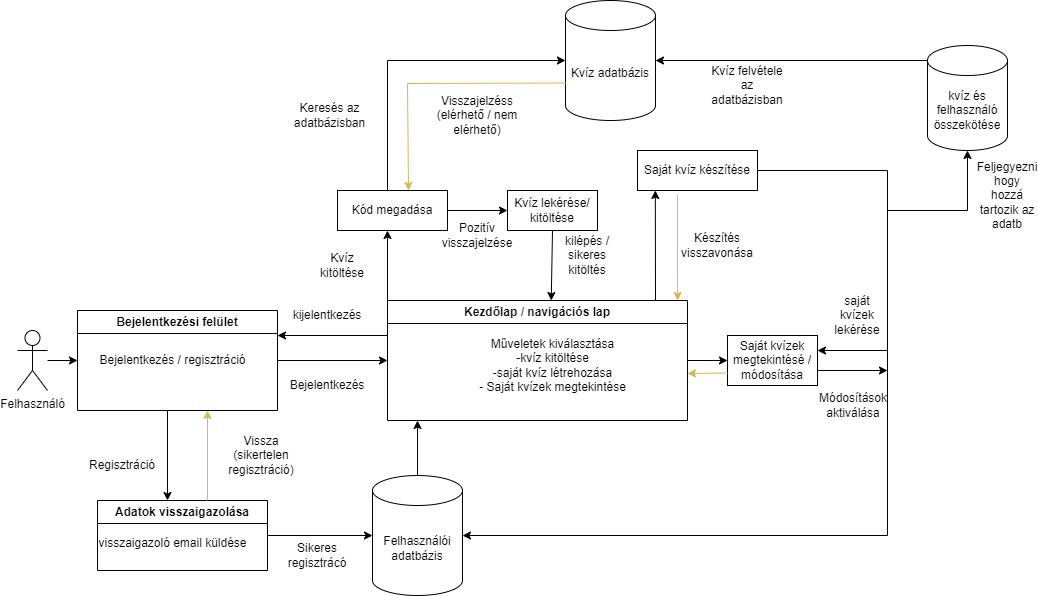
\includegraphics[width=1\textwidth]{web.png}
    \caption{A weboldal kezdetleges kinézete}
    \label{fig:A weboldal kezdetleges kinézete}
\end{figure}

\subsection{Bejelentkező / regisztrációs felület}
Ahogy valaki csatlakozik a weboldalunkhoz ez a felület fogja köszönteni. Mivel minden felhasználókat azonosítani kell tudnunk, azért lesz erre szükség. A regisztrációval egy új fiókot hozhatunk majd létre, amit majd egy e-mailes visszaigazolás követ majd. Ha az sikerült akkor a felhasználónk bekerül a „rendszerbe” és igénybe veheti a weboldal lehetőségeit.
\subsection{Kezdőlap}
Itt tudja majd a felhasználó, a bejelentkezés / regisztráció után az oldal adta lehetőségeket elérni, amik:
\begin{itemize}
	\item \textit{\underline{Teszt kitöltése:}} Egy kód segítségével történik, mely minden kvíz létrehozásánál generálódik, férhetünk majd hozzá az adott teszthez (esetleg még akár megosztás alapon is). Így tudjuk majd azt limitálni, hogy csak az álltalunk célzott közönség töltse ki.
	\item \textit{\underline{Saját kvíz készítése:}} Itt tudunk majd saját kvízeket létrehozni, valamint különböző szabályokat alkalmazni a kérdésekre, magára az egészre, ilyen lesz, például az, hogy több helyes választ lehetőségből egyet, vagy akár többet is belerakhat a válaszok közé. Ugyanígy működhetnek a rossz válaszok, mint például megadunk 10 rossz választ s azt mondjuk, hogy a kérdésre max 5 válasz lehet adni, így 1 (vagy többet attól függően hogy mennyit adtunk meg, de egyet biztosan) jót és 5 véletlenszerű rossz választ majd.
	\begin{figure}[h]
    		\centering
    		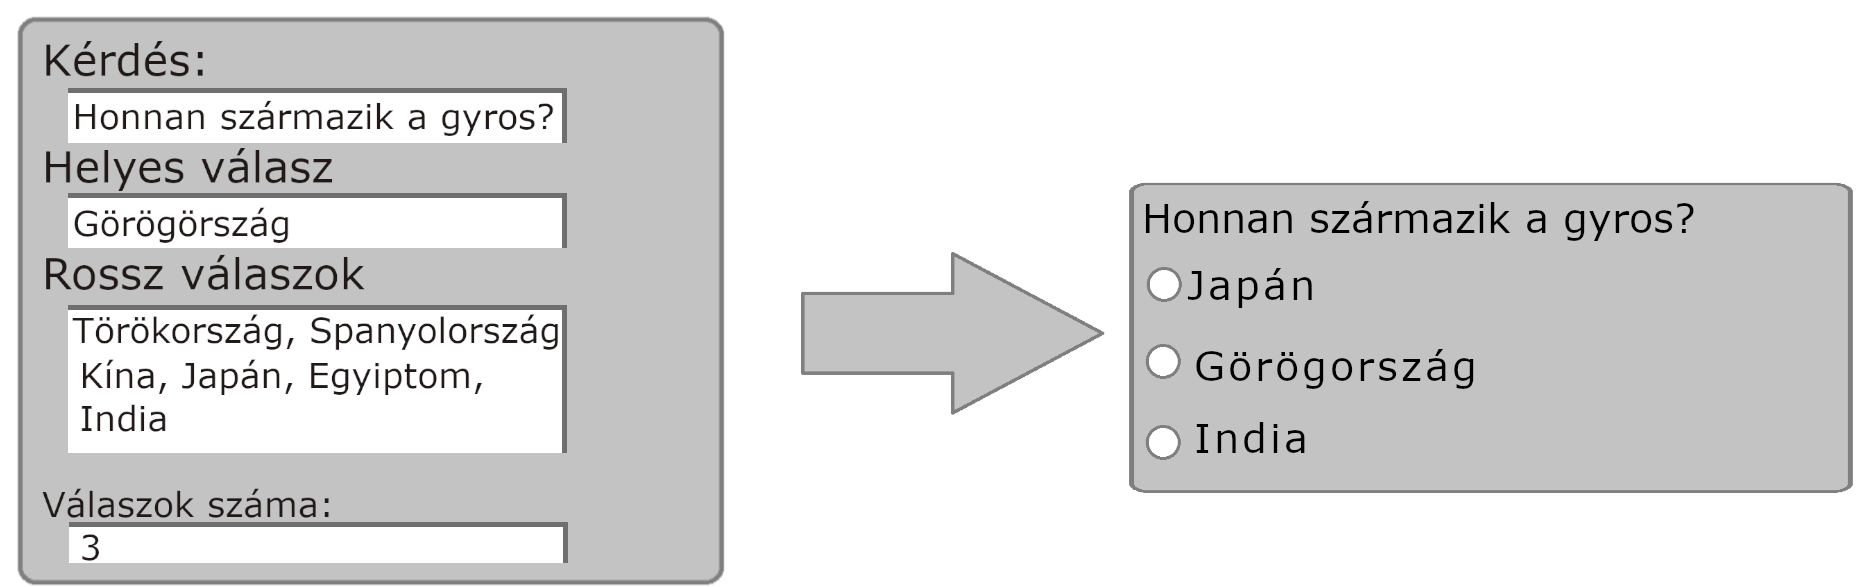
\includegraphics[width=1\textwidth]{MORE_QUEST.png}
    		\caption{Minta a random válaszlehetőség választására}
    \label{fig:Minta a random válaszlehetőség választására}
\end{figure}
Egy másik sokkal effektívebb randomizálási módszer lehet amit úgy neveztem el, hogy TAG-olás. Az egésznek az a lényege, hoy veszek egy speciális kódsorozatot, mint például a \$[Felhasználó álltal megadott azonosító]\$ majd az azonosító alapján egy ellőre definiált kifejezés / szóhalmazból választ oda egyet random például:
\begin{figure}[h]
    			\centering
    			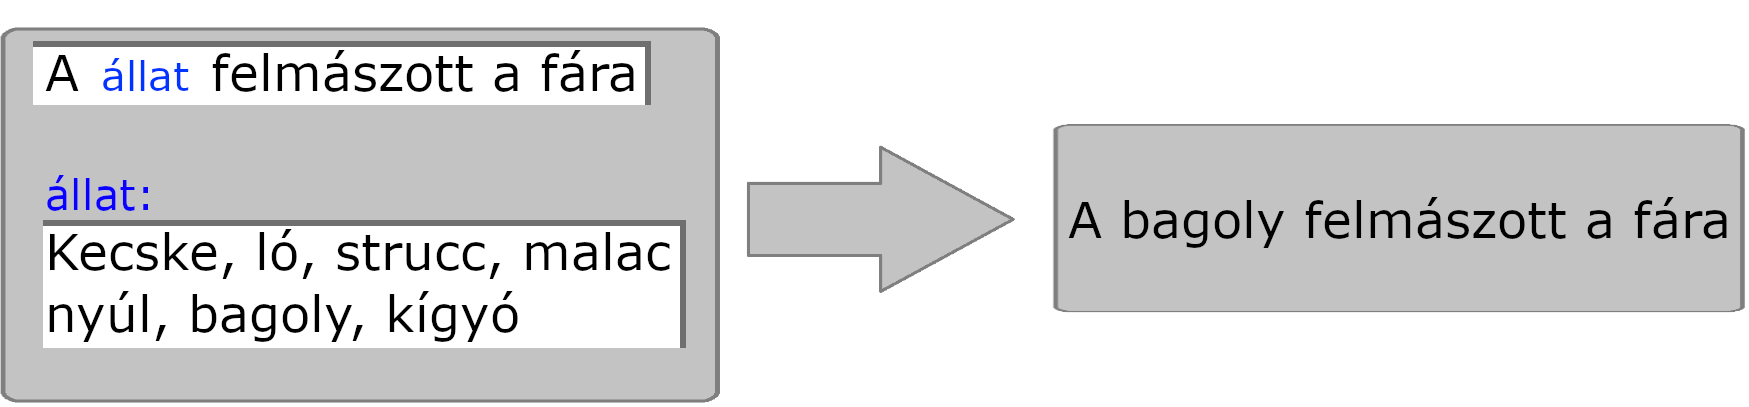
\includegraphics[width=0.7\textwidth]{tag.png}
    			\caption{Példa a TAG-olásra}
    			\label{fig: Példa a TAG-olásra}	
		\end{figure}
Ez a megoldás azért lehet jobb mint az első, mert itt továbbra is megvan az a lehetőségünk, hogy a helyes illetve a helytelen válaszok valamiféle összhangban legyenek egymással, hogy megzavarjuk azt a személyt akik a tesztünket töltik ki. Úgy tervezem, hogy amint az algoritmus érzékeli, hogy mi TAG-olást akarunk használni létrehoz annak a tagnak az azonosítóójával egy új input mezőt, ahova írhatjuk majd az extra kifejezéseinket. Mivel a keverési ötleteim megvalósításához legegyszerűbb lesz különböző tömböket használon, így a kvízek JSON-ként lesznek majd tárolva.
	\item \textit{\underline{Saját kvízek megtekintése/módosítása}} Itt tudjuk majd a kvízeinket törölni, vagy megtekinteni a beküldött erdményeket. (Mint például hányan töltötték ki a kvízt, eredmények stb)
	\item \textit{\underline{Adatbázis:}} A felhasználókat és a hozzájuk tartozó kérdéssorokat valahol tárolni is kellen, erre fogjuk használni az adatbázisokat:
		\begin{figure}[h]
    			\centering
    			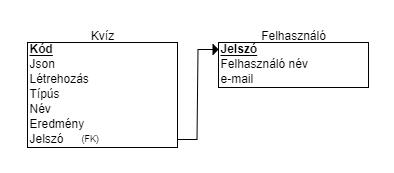
\includegraphics[width=0.5\textwidth]{database.png}
    			\caption{Egy egyszerűsített adatbázis}
    			\label{fig:Egy egyszerűsített adatbázis}	
		\end{figure}
		Itt látatjuk a fontosabb elemeit egy Relációs diagrammban. Egy ember akár több kvízzel is rendelkezhet, de egy kvíznek csak egy gazdája lehet majd. A kvízeket majd JSON-formátumba tervezem tárolni, hogy könnyen, gyorsan lehessen őket kezelni a műveletek miatt, mint randomizálás stb. Jelenleg a két entitást jelszó alapján kötöm össze ami eléggé nagy biztonsági probléma lehet. Úgyhogy valószínűleg a jövőben egy hosszú, random generált kód alapján is számon lesznek tartva a felhasználók.
\end{itemize}

\section{Lehetséges problémák}
\subsection{Kihasználatlanság}
A legszenbetűnőbb probléma az, amit akár a hybrid meghajtású autóknál is megfigyelhetünk. Az emberek akik majd használni foglyák a weboldalt, valószínűleg nem vesznek majd annyi fáradságot, hogy megtanulják a készítő-felület összes lehetőségét. Nem várhatjuk el attól például attól az egyetemi professzortól hogy a microsoft űrlapok kezelésének a megértése után egy talán komplexebb felületet is megtanuljon, ez ahhoz fog vezetni hogy hiába vannak implementálva érdekes funkciók, azok kihasználatlanok fognak maradni.
\subsection{Csalások}
A másik nagyon fontos kérdés a csalásokra vonatkozik. Ugyanis, manapság a diákság között eléggé sok jól működő módszer van, amivel az ilyen típusú oldalakat elég könnyen kicselezhetik. Például:
\begin{itemize}
	\item\textbf{Adatok átírása}: Ez amióta léteznek kvíz, weboldalak azóta probléma az, hogy bárki akár egy kicsi tudással is a weboldalak működéséről és a "vizsgálat" segítségével átírhatja a kapott eredményeket. Erre oda kell figyelni az implementálásnál, hogy a felhasználó oldalán ne legyen adatkezelés, viszont ez a folyamatos kliens-szerver jobban terhelheti a szerverünket.
	\item\textbf{AI használata:} Manapság egyre inkább nagyobb problémát jelent az AI elterjedése. A kitöltő ember ha csalni akar, egyszerűen kimásolja a kérdést és a válaszokat, átadja az álltala használt nyelvi modellnek, ő meg kiadja a (elég nagy eséllyel) helyes megfejtéseket. Ezt kicsit lehet gátolni időkorlátokkal (például 10s minden másodpercre) de ezzel diszkriminálhatjuk a nem olyan gyorsan olvasó, esetleg szöveget nehezebben megértő felhasználóinkat. Az egyik, szerintem hatékonyabb megoldás, a kérdések és válaszok képpé átformázása a kvíz betöltésekor (például SVG) ezálltal nehezebbíthetnénk a dolgot, ugyanis sok ingyenes mesterséges inteligencia nem alkalmas képek elemzésére. Habár ez a funkció egyre több modellben kezd feltünögetni, valamint a fizetősek sincsenek olyan megfizethetetlen áron, így ez se lesz 100\%-os megoldás.
\end{itemize}

\bibliographystyle{plain}
\bibliography{references}

\end{document}
